% =====================================================================================================
% Question 2 -- Can price signals achieve what the central dispatch does?                  (Alejandro)
% Code: src/pricing.py (model), src/q2.py (experiments). Every number below comes from one of
%   python main.py --q2 validate | steps | indifference | sensitivity
% =====================================================================================================
In Question~1 the manager could switch every appliance of the community on and off.
We now take this power away.
Once a day, after the day-ahead prices and the cap are known, the manager posts one internal price $x_t$ for every hour, the same for all members, and each member then schedules its own appliances against these prices, exactly as the consumer of Assignment~1 did.
The manager still pays the DSO for the exchange at the connection point and knows perfectly how every member responds.
We ask how much of the value and flexibility of $\mathcal{C}$ these prices can recover, whether the same prices can also balance the manager's budget and leave every member better off than alone, and what these two requirements cost the community.

\subsection{Models}

\subsubsection{Members: best response to posted prices}
Member $i$ keeps the feasible set $\mathcal{X}_i$ of~\eqref{eq:member} and the own cost $K_i$ of~\eqref{eq:owncost}.
Given the posted prices $x=(x_t)_{t\in\mathcal{T}}$, it chooses its decisions $y_i$ (load, deviations, PV and battery) by solving
\begin{equation}\label{eq:DP_member}
\mathcal{F}_i(x):\qquad \min_{y_i\in\mathcal{X}_i}\ J^{\mathcal{DP}}_i=\sum_{t\in\mathcal{T}}x_t\,q_{i,t}+K_i .
\end{equation}
Compared with $\mathcal{R}$, the member no longer has a meter of its own.
The import and export variables, the balance~\eqref{eq:R_bal}, the tariffs and the penalty all leave its problem, and the two prices $p^{\mathrm{imp}}_t>p^{\mathrm{exp}}_t$ become a single price $x_t$ on its net consumption.
Since the price only enters the objective, the manager changes what each member optimizes but never what it can do.

Buying and selling at the same price has three consequences.
A kWh of PV is worth $x_t$ whether it is used at home, sold to a neighbour or exported, so self-consumption earns no premium and the PV runs whenever $x_t\geq c^{\mathrm{PV}}$.
The battery only reacts to price differences and moves energy from hour $t$ to hour $s$ when $\eta^{\mathrm{ch}}\eta^{\mathrm{dis}}x_s>x_t$.
For the manager, the budget of hour $t$ becomes $(x_t-\tilde{p}^{\mathrm{imp}}_t)P^{\mathrm{imp}}_t-(x_t-\tilde{p}^{\mathrm{exp}}_t)P^{\mathrm{exp}}_t-\alpha^{\mathrm{DSO}}P^{\mathrm{exc}}_t$, so it collects a rent whenever the price of an importing hour exceeds the discounted import price.

Problem~\eqref{eq:DP_member} is a linear program, and its KKT conditions are listed in Appendix~A.
For the load they give the three regimes of Assignment~1.
With $\mu^E_i$ the multiplier of the daily minimum, the load stays at its reference while $|x_t-\mu^E_i|<c^L_i$ and moves to one of its bounds otherwise.
When $|x_t-\mu^E_i|=c^L_i$ the member is indifferent, and its best response is a set rather than a single schedule.

\subsubsection{Manager: welfare-maximizing prices}
The manager chooses the prices and the exchange at the connection point, anticipating how every member will respond:
\begin{subequations}\label{eq:DP}
\begin{align}
\min_{\substack{x,\ P^{\mathrm{imp}},P^{\mathrm{exp}},P^{\mathrm{exc}}\geq 0\\ (y_i)_{i\in\mathcal{M}}}}\quad & J^{\mathcal{DP}}=\sum_{t\in\mathcal{T}}\Big(\tilde{p}^{\mathrm{imp}}_tP^{\mathrm{imp}}_t-\tilde{p}^{\mathrm{exp}}_tP^{\mathrm{exp}}_t+\alpha^{\mathrm{DSO}}P^{\mathrm{exc}}_t\Big)+\sum_{i\in\mathcal{M}}K_i \label{eq:DP_obj}\\
\text{s.t.}\quad & \eqref{eq:C_bal},\ \eqref{eq:C_cap}, \qquad \underline{x}_t\leq x_t\leq\overline{x}_t \qquad \forall t\in\mathcal{T}, \label{eq:DP_upper}\\
& y_i\in\arg\min\ \mathcal{F}_i(x) \qquad \forall i\in\mathcal{M}. \label{eq:DP_lower}
\end{align}
\end{subequations}
The objective~\eqref{eq:DP_obj} is the welfare of $\mathcal{C}$.
The internal payments $\sum_tx_tq_{i,t}$ are transfers between the members and the manager, so they cancel out.
The manager therefore acts in the interest of the community but is indifferent to how the welfare is shared: the prices only matter through the dispatch they induce.
We bound the prices by $\underline{x}_t=0$, since a negative price would pay members to waste energy, and by $\overline{x}_t=\max_s\tilde{p}^{\mathrm{imp}}_s+\alpha^{\mathrm{DSO}}$, since no kWh can ever cost the community more.
Both bounds contain every value that $\lambda_t$ took in Question~1.

Two properties follow directly from this formulation.
First, $J^{\mathcal{DP}}\geq J^{\mathcal{C}}$, because~\eqref{eq:DP_lower} restricts the dispatch of $\mathcal{C}$ to the responses the members are willing to give.
Second, the dual prices $\lambda_t$ of~\eqref{eq:C_bal} attain $J^{\mathcal{C}}$.
The KKT conditions of $\mathcal{C}$ separate member by member when every member sees $\lambda_t$, so the dispatch of $\mathcal{C}$ is a best response of every member to these prices.
This is the competitive-equilibrium argument behind uniform marginal pricing in market clearing.
One uniform price per hour is therefore enough to reproduce $\mathcal{C}$.
That price is not unique, though, and nothing in~\eqref{eq:DP} protects the members.

\paragraph{Solution concept.}
Problem~\eqref{eq:DP} is a Stackelberg game in which the manager leads and the members follow.
When a member is indifferent, \eqref{eq:DP_lower} lets the manager pick the response it prefers among the member's optimal ones, which makes~\eqref{eq:DP} an optimistic bilevel problem.
We return to this assumption in Section~\ref{sec:q2_indifference}.

\subsubsection{Single-level reformulation}
Each $\mathcal{F}_i(x)$ is a linear program, so its KKT conditions describe its set of optimal responses exactly and can replace~\eqref{eq:DP_lower}.
The stationarity conditions are linear in the prices and the duals, because $x_t$ never multiplies a variable there.
What remains non-convex are the complementarity conditions $0\leq a\perp b\geq0$.
We write each of them with one binary $u$ as $a\leq M^{\mathrm{P}}u$ and $b\leq M^{\mathrm{D}}(1-u)$.
The constants $M^{\mathrm{P}}$ follow from the bounds of $\mathcal{X}_i$.
For the load and the PV, the constants $M^{\mathrm{D}}$ follow from the KKT conditions themselves, so they cut off no response (Appendix~A).
For the battery we use $M^{\mathrm{D}}=50$~DKK/kWh and check after every solve that no dual reaches it.
The objective~\eqref{eq:DP_obj} contains no product of a price and a quantity, so the variant with the contract only, $\mathcal{DP}^{\mathrm{cap}}$, needs no further step.
The requirements below do contain the payments $\Pi_i=\sum_tx_tq_{i,t}$, which are bilinear.
Strong duality of $\mathcal{F}_i(x)$ gives $\Pi_i+K_i=\Phi_i(\xi_i)$, the dual objective of member $i$ (Appendix~A).
$\Phi_i$ is linear in the duals $\xi_i$, because the prices only appear in the dual constraints.
The result is a mixed-integer linear program.

\subsubsection{Requirements and variants}
\paragraph{Budget balance.}
The manager is a non-profit entity, so the payments it collects must equal the DSO bill $D$ of~\eqref{eq:bill}:
\begin{equation}\label{eq:DP_BB}
\sum_{i\in\mathcal{M}}\big(\Phi_i(\xi_i)-K_i\big)=D .
\end{equation}
We use an equality rather than an inequality because~\eqref{eq:DP_obj} does not see the transfers: with an inequality, the surplus would be arbitrary among the optimal solutions.
The equality has a side effect, however.
The manager could balance its budget by wasting money at the meter, importing and exporting in the same hour or paying the penalty below the cap.
Two binaries per hour, $u_t$ and $z_t$, rule this out through $P^{\mathrm{imp}}_t\leq Mu_t$, $P^{\mathrm{exp}}_t\leq M(1-u_t)$, $P^{\mathrm{exc}}_t\leq Mz_t$ and $P^{\mathrm{exc}}_t\leq P^{\mathrm{imp}}_t-\overline{P}^{\mathrm{DSO}}_t+M(1-z_t)$.

\paragraph{Individual rationality.}
No member may end up worse off than in its benchmark:
\begin{equation}\label{eq:DP_IR}
\Phi_i(\xi_i)\leq J^{\mathrm{bench}}_i \qquad \forall i\in\mathcal{M}.
\end{equation}
Both sides contain the same components as~\eqref{eq:ir}: payments, disutility and PV production cost, with the same end-of-day state of charge.
Our benchmark is $\mathcal{R}$, because signing nothing is the one option every member always keeps.
A stricter variant, $\mathrm{IR}^{\mathcal{RI}}$, uses $\min(J^{\mathcal{R}}_i,J^{\mathcal{I}}_i)$ under the same contract terms.

\paragraph{Infeasibility.}
A single price per hour may not be able to satisfy both requirements, so we extend the same model in two ways.
In the soft variant $\mathcal{DP}^{\mathrm{BB,IR,soft}}$, each member's benchmark in~\eqref{eq:DP_IR} is relaxed by a slack $s_i\geq0$, and $\rho\sum_is_i$ with $\rho=10^3$ is added to~\eqref{eq:DP_obj}.
The members with $s_i>0$ are the ones blocking, and $\sum_is_i$ is what would have to be given up to satisfy them.
With price discrimination, $x_t$ is replaced by one price vector per asset class ($\mathcal{DP}^{\cdot,\mathrm{asset}}$, four vectors) or per member ($\mathcal{DP}^{\cdot,\mathrm{member}}$), which tells us how many price signals the requirements actually need.
Table~\ref{tab:DP_variants} summarizes the variants.

\begin{table}[htbp]
\centering
\caption{Variants of the pricing problem, all built as one parametrized model (\texttt{src/pricing.py}).}
\label{tab:DP_variants}
\small
\begin{tabular}{@{}lll@{}}
\toprule
Variant & Constraints added to \eqref{eq:DP} & Prices\\
\midrule
$\mathcal{DP}^{\mathrm{cap}}$ & -- & one per hour\\
$\mathcal{DP}^{\mathrm{BB}}$ & \eqref{eq:DP_BB} and the binaries $u_t,z_t$ & one per hour\\
$\mathcal{DP}^{\mathrm{BB,IR}}$ & \eqref{eq:DP_BB}, \eqref{eq:DP_IR} & one per hour\\
$\mathcal{DP}^{\mathrm{BB,IR,soft}}$ & \eqref{eq:DP_BB}, \eqref{eq:DP_IR} relaxed by $s_i$ & one per hour\\
$\mathcal{DP}^{\mathrm{BB,IR,asset}}$, $\mathcal{DP}^{\mathrm{BB,IR,member}}$ & \eqref{eq:DP_BB}, \eqref{eq:DP_IR} (or relaxed) & per asset class, per member\\
\bottomrule
\end{tabular}
\end{table}

\subsection{Problem class, size and validation}
Every variant is a mixed-integer linear program.
On the base case it has 10\,296 variables, 2\,952 of them binary (one per complementarity pair, plus 48 with budget balance), and 10\,248 constraints.
Writing the complementarity with big-M matters for the solution time.
With the constants above, Gurobi solves $\mathcal{DP}^{\mathrm{cap}}$ to optimality in about one second without a warm start, whereas with SOS1 constraints the gap was still 43\,\% after 300~s.

We validate the model in three ways (\texttt{python main.py --q2 validate}).
First, $\mathcal{DP}^{\mathrm{cap}}$ reaches $J^{\mathcal{C}}=372.16$~DKK exactly.
Second, the reformulation is exact at the solution: the strong-duality and complementarity residuals are below $10^{-9}$, and re-solving every member's own linear program at the posted prices gives back the cost the manager anticipated.
Third, at $x=\lambda$ the dispatch of $\mathcal{C}$ is a best response of every member, as the theory predicts.
The validation also shows that the optimal prices are far from unique.
Depending on the solver's path, $\mathcal{DP}^{\mathrm{cap}}$ returns prices that leave the manager with a surplus anywhere between about 40 and 170~DKK, all for the same welfare.

% ---------------------------------------------------------------------------------------------------
\subsection{Metrics}
Table~\ref{tab:DP_metrics} lists the metrics of this question.
They compare each variant with $\mathcal{C}$, the efficient benchmark, and with $\mathcal{R}$ and $\mathcal{I}$, the members' alternatives.

\begin{table}[htbp]
\centering
\caption{Metrics of Question 2, with their reference, point of view and sign.}
\label{tab:DP_metrics}
\small
\begin{tabularx}{\textwidth}{@{}lXlll@{}}
\toprule
Metric & Definition & Unit & Reference & Point of view\\
\midrule
Efficiency loss & $J^{\mathcal{DP}}-J^{\mathcal{C}}$, positive when a requirement costs welfare & DKK & $\mathcal{C}$ & community\\
Energy above the cap & $X=\sum_t\max(0,P^{\mathrm{imp}}_t-\overline{P}^{\mathrm{DSO}}_t)$ & kWh & 0 (as in $\mathcal{C}$) & DSO\\
Budget & $B=\sum_i\Pi_i-D$, positive when the manager keeps a surplus & DKK & 0 & manager\\
Member gain & $V_i=J^{\mathcal{R}}_i-J^{\mathcal{DP}}_i$, positive when $i$ gains by signing & DKK & $\mathcal{R}$ & member\\
Members worse off & number of members with $J^{\mathcal{DP}}_i>J^{\mathcal{R}}_i$ (or $>J^{\mathcal{I}}_i$) & -- & $\mathcal{R}$, $\mathcal{I}$ & members\\
IR violation & $\sum_is_i$ in the soft variants, and the blocking members ($s_i>0$) & DKK & 0 & members\\
\bottomrule
\end{tabularx}
\end{table}

% ---------------------------------------------------------------------------------------------------
\subsection{Base case: cap, budget balance and individual rationality}\label{sec:q2_steps}
% Command: python main.py --q2 steps
Table~\ref{tab:DP_steps} summarizes the three steps on the base case.
Figure~\ref{fig:q2_prices} shows the posted prices and Figure~\ref{fig:q2_members} how each member fares.

\begin{table}[htbp]
\centering
\caption{The three steps on the base case. Loss against $\mathcal{C}$, budget and IR violation in DKK; energy above the cap in kWh. The MILPs were stopped after 300~s where a gap is given.}
\label{tab:DP_steps}
\small
\begin{tabular}{@{}lrrrrrrl@{}}
\toprule
Variant & Loss & Above cap & Budget $B$ & Worse off & Worse off & IR viol. & Gap\\
 & vs $\mathcal{C}$ & $X$ & & than $\mathcal{R}$ & than $\mathcal{I}$ & $\sum_is_i$ & \\
\midrule
$\mathcal{C}$, dual price $\lambda_t$ & -- & 0.00 & 163.77 & 13 & 8 & -- & --\\
$\mathcal{DP}^{\mathrm{cap}}$ & 0.00 & 0.00 & 39.61 & 8 & 7 & -- & 0\\
$\mathcal{DP}^{\mathrm{BB}}$ & 0.02 & 0.00 & 0.00 & 7 & 4 & -- & $10^{-4}$\\
$\mathcal{DP}^{\mathrm{BB,IR}}$ & \multicolumn{7}{l}{no feasible point found within 300~s}\\
$\mathcal{DP}^{\mathrm{BB,IR,soft}}$ & 10.49 & 1.37 & 0.00 & 5 & 2 & 10.61 & 97\,\%\\
$\mathcal{DP}^{\mathrm{BB,IR,asset}}$ & 1.22 & 0.21 & 0.00 & 0 & 2 & 0.00 & 0.3\,\%\\
$\mathcal{DP}^{\mathrm{BB,IR,member}}$ & 0.00 & 0.00 & 0.00 & 0 & 2 & 0.00 & 0\\
\bottomrule
\end{tabular}
\end{table}

\paragraph{Step 1: the cap only.}
With one price per hour, the manager recovers the whole value of $\mathcal{C}$: $J^{\mathcal{DP}^{\mathrm{cap}}}=J^{\mathcal{C}}$, and no energy is imported above the cap.
What makes this possible is a property of the members rather than of the prices: they are price-takers with linear, hence convex, problems, so the dual price of $\mathcal{C}$ supports its dispatch member by member.
The price is pinned to the discounted import price in hours 17 and 22 and to the discounted export price in the export hours 18--20.
In the 18 capped hours it is set by the cap and a marginal member (Section~\ref{sec:q2_indifference}).
This first step, however, says nothing about who pays.
The solver returned prices that leave the manager a surplus of 39.6~DKK, whereas at $\lambda_t$ it keeps the whole congestion rent of 163.8~DKK, and with either price eight or more members are worse off than without a contract.

\paragraph{Step 2: budget balance.}
Returning the rent costs almost no welfare: 0.02~DKK, which is within the remaining optimality gap.
The way the manager achieves it is telling (Figure~\ref{fig:q2_prices}).
It keeps prices close to $\lambda_t$ in almost every hour, and raises them to 10.6 and 12.6~DKK/kWh in hours 19 and 20.
In those hours the community exports and every battery already discharges at full power, so nobody can react further, and the higher price only moves money.
That money goes to whoever sells in those hours, above all the members with both PV and a battery (Figure~\ref{fig:q2_members}).
Seven members are still worse off than in $\mathcal{R}$, six of them without PV.
This is the first sign of the limitation of a uniform price: every krone handed back through the price of an hour also goes to everyone else who trades in that hour.

\paragraph{Step 3: individual rationality.}
With one price per hour, the solver found no prices meeting both requirements within 300~s, nor could it prove that none exist.
The soft variant gives the best compromise it found.
The individual rationality is violated by 10.6~DKK in total, borne by C2, C3, C4, C3\_B and C4\_B, at a welfare loss of 10.5~DKK and 1.4~kWh above the cap.
To protect these members the manager has to flatten the prices of the capped hours (red line in Figure~\ref{fig:q2_prices}), which lets some flexible load back into them.
The blocking members are the stiff loads without PV.
They buy their reference profile precisely in the hours where the price must stay high to keep the flexible members out, and a single price cannot tell the two groups apart.

Price discrimination removes this conflict.
With one price vector per asset class, both requirements hold at a welfare loss of 1.2~DKK, about 5\,\% of the value of $\mathcal{C}$, and with one price per member they hold at no loss at all.
In both cases the objective still leaves the split of the community's gain open: many price vectors satisfy the requirements, and the solver simply returns one of them (Figure~\ref{fig:q2_members}).
Choosing among them would need an explicit fairness criterion, which neither requirement provides.

\begin{figure}[htbp]
\centering
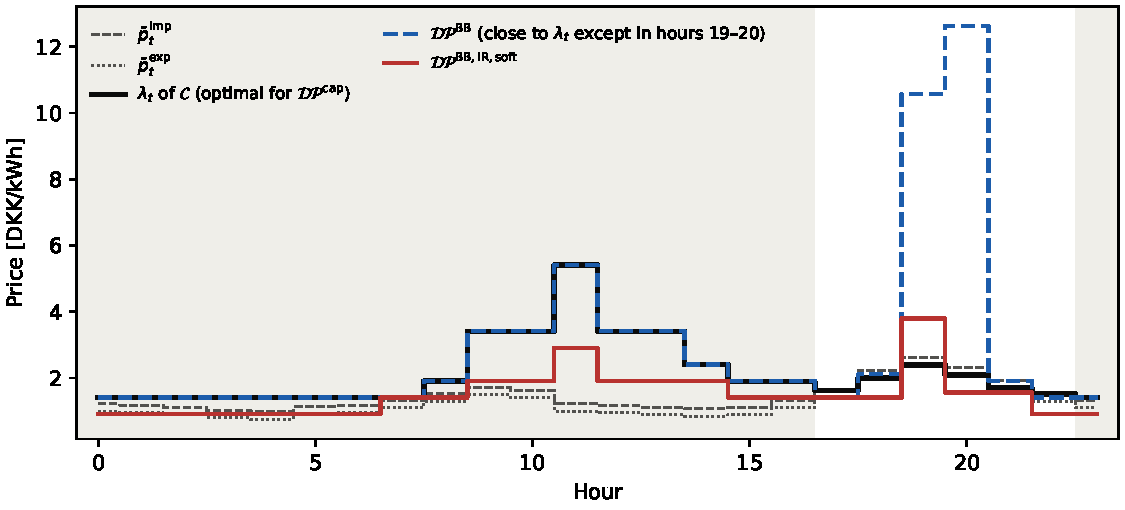
\includegraphics[width=0.85\linewidth]{figures/Q2/q2_prices.pdf}
\caption{Posted prices on the base case (capped hours shaded). Budget balance keeps the prices of $\mathcal{C}$ and returns the rent through two export hours; individual rationality flattens the prices of the capped hours.}
\label{fig:q2_prices}
\end{figure}

\begin{figure}[htbp]
\centering
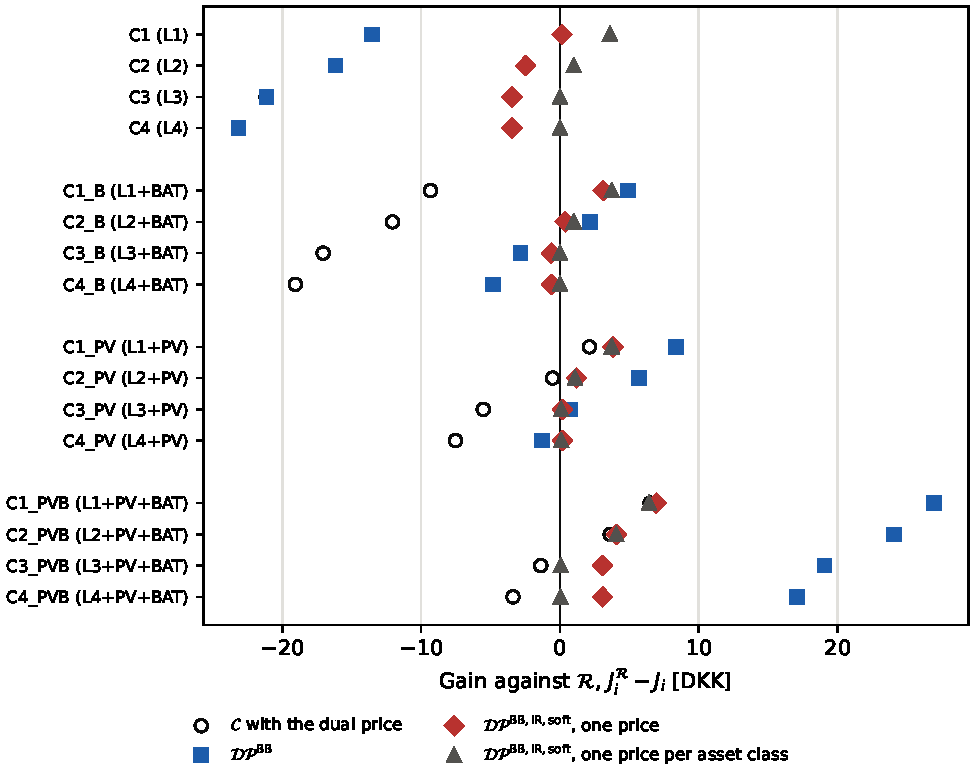
\includegraphics[width=0.72\linewidth]{figures/Q2/q2_members.pdf}
\caption{Gain of every member against $\mathcal{R}$, grouped by assets and ordered by slope. Budget balance alone passes the rent to the PV and battery owners; with one price per asset class nobody is worse off than without a contract.}
\label{fig:q2_members}
\end{figure}

% ---------------------------------------------------------------------------------------------------
\subsection{Indifference}\label{sec:q2_indifference}
% Command: python main.py --q2 indifference
With a linear disutility, a member's best response is a set whenever the price of an hour lies exactly $c^L_i$ away from its internal value $\mu^E_i$.
The optimal prices sit precisely at these points.
In the capped hours, $\lambda_t$ is set by the marginal member.
When a load is marginal, the price equals the night price of 1.41~DKK/kWh plus $2c^L$ of its class (1.91, 2.41, 3.41 and 5.41~DKK/kWh for L1 to L4), because a load only moves a kWh from hour $t$ to hour $s$ if $x_t-x_s>2c^L_i$.
When a battery is marginal, as in hours 15--16, the price is 1.895~DKK/kWh.
At these prices 220 of the 384 member-hours are indifferent, and there are indifferent members in every hour where the cap binds.

The single-level model breaks every one of these ties in the manager's favour, and that is what makes it optimistic.
In practice a member has no reason to choose the schedule the manager has in mind.
If all members broke their ties the other way, hour by hour, the import could exceed the cap in all 18 capped hours, and the manager would pay the penalty $\alpha^{\mathrm{DSO}}$ although every member behaved optimally.
A pessimistic manager would instead price slightly inside each tie, so that every response becomes unique, at a small cost in welfare or budget.
Question~3 returns to this exposure, since with uncertain preferences the members may end up on the wrong side of a tie.

% ---------------------------------------------------------------------------------------------------
\subsection{Sensitivity to the cap}\label{sec:q2_sensitivity}
% Command: python main.py --q2 sensitivity
The base case is a single contract.
Since both requirements are about sharing the congestion rent, the tightness of the cap is the natural dimension to vary (Table~11~c).
We solved the three steps for cap factors $f$ between 1.1 and 4.0, keeping $\beta^{\mathrm{DSO}}=0.75$ and $\alpha^{\mathrm{DSO}}=10$~DKK/kWh fixed (Figure~\ref{fig:q2_sensitivity}).
Before running the study we expected a looser cap to lower the rent, make budget balance cheaper, and turn individual rationality from infeasible into feasible at some threshold.

The results confirm this and place the threshold between $f=1.3$ and $f=1.4$.
From $f=1.4$ on, a single price per hour meets both requirements at no cost in welfare.
The threshold has a clear cause in the merit order of Section~\ref{sec:q2_indifference}.
At $f=1.3$ the cap still forces the stiffest class, L4, to shift 0.4~kWh out of hour 11, which lifts the price of that hour to 5.41~DKK/kWh.
At $f=1.4$ no L4 load needs to move, so the highest price drops to 3.23~DKK/kWh (now set by L3) and the rent halves from 164 to 84~DKK.
The stiff members then pay little enough in the capped hours for one price to leave all of them better off.
Put simply, a uniform price fails as soon as the cap reaches the stiffest members.

Budget balance follows a related logic.
It stays almost free as long as the rent can be handed back through the export hours, where nobody reacts to the price, that is, as long as the rent does not exceed $\sum_t(\overline{x}_t-\lambda_t)P^{\mathrm{exp}}_t$.
In the base case the rent is 164~DKK against a margin of 228~DKK.
At $f=1.2$ the rent of 233~DKK exceeds the margin of 205~DKK, and returning it costs 6.9~DKK of welfare.
This threshold depends on the price bound $\overline{x}_t$, which is therefore a modelling choice with visible consequences.

At the tight end, individual rationality becomes impossible altogether.
Summing~\eqref{eq:DP_IR} over all members under budget balance gives $\sum_is_i\geq J^{\mathcal{DP}}-J^{\mathcal{R}}\geq-V^{\mathcal{C}}$.
At $f=1.1$ the community loses 7.9~DKK even under central dispatch, so no prices, not even one per member, can leave every member better off.
The best uniform price we found there leaves 87~DKK of violation, and every member without PV is blocking.
Prices per asset class reduce the violation considerably, to 23~DKK at $f=1.1$ and 8~DKK at $f=1.2$, and to zero in the base case.
Where the gap is still open, these soft results are the best points found, so they are upper bounds on the smallest possible violation.

\begin{figure}[htbp]
\centering
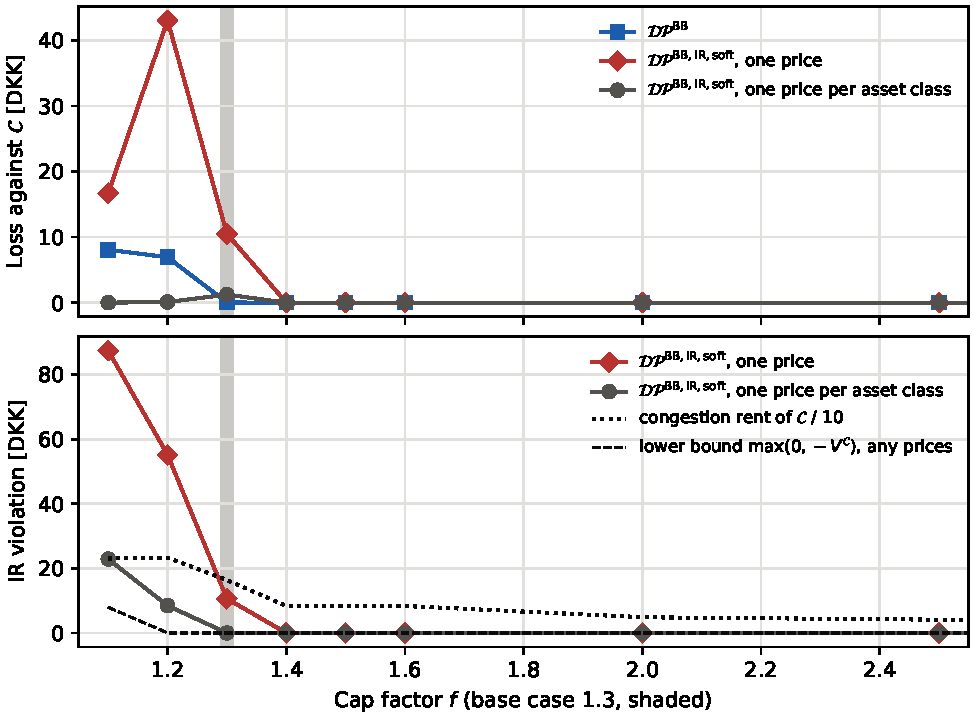
\includegraphics[width=0.75\linewidth]{figures/Q2/q2_sensitivity.pdf}
\caption{Efficiency loss (top) and IR violation (bottom) along the cap factor. One price per hour meets both requirements from $f=1.4$, once the cap no longer forces the stiffest members to move; below $f\approx1.15$ no prices can. Points with $f\leq1.3$ are the best solutions found within 120--240~s; for $f>2.5$ all curves stay at zero.}
\label{fig:q2_sensitivity}
\end{figure}

\subsection{Conclusions and recommendation}
Prices alone can reproduce the central dispatch.
Because the members are price-takers with linear problems, one price per hour recovers the whole value and flexibility of $\mathcal{C}$.
This holds only in the optimistic sense, however: the optimal prices sit on the members' ties, and a manager who cannot count on every tie being broken its way should price slightly inside them.

Of the two requirements, budget balance is almost free in the base case, whereas individual rationality is the one a uniform price struggles with.
The stiff members without PV need low prices in exactly the hours where the flexible members need high ones, and a single price cannot serve both.
In the base case we found no uniform price that leaves every member better off than without a contract.
One price per asset class achieves it for 1.2~DKK of welfare, and one price per member at no cost at all.
Whether a uniform price is enough depends on the contract.
With a loose cap it is, and with a cap so tight that the community as a whole loses, no prices can make every member better off.

We therefore recommend that the manager impose both requirements.
Without them, the price either over-collects, as in Question~1, or hands the rent back to the members who happen to sell in a few export hours.
When the cap is tight, the manager should differentiate the price by asset class, which needs only four price signals and costs little welfare.
For the DSO this is part of the trade-off identified in Question~1: a looser cap makes a simple uniform tariff possible, but removes less congestion.
